\documentclass[11pt]{exam}
\usepackage[margin=1in]{geometry}
\usepackage{amsfonts, amsmath, amssymb, amsthm}
\usepackage{mathtools}
\usepackage{enumerate}
\usepackage{listings}
\usepackage{colortbl}
\usepackage{float}
\usepackage[colorlinks,linkcolor=blue]{hyperref}

% in order to compile this file you need to get 'header.tex' from
% Canvas and change the line below to the appropriate file path
%%% theorems

\theoremstyle{plain}            % following are "theorem" style
\newtheorem{theorem}{Theorem}[section]
\newtheorem{lemma}[theorem]{Lemma}
\newtheorem{corollary}[theorem]{Corollary}
\newtheorem{proposition}[theorem]{Proposition}
\newtheorem{claim}[theorem]{Claim}
\newtheorem{fact}[theorem]{Fact}
\newtheorem{openproblem}[theorem]{Open Problem}

\theoremstyle{definition}       % following are def style
\newtheorem{definition}[theorem]{Definition}
\newtheorem{conjecture}[theorem]{Conjecture}
\newtheorem{example}[theorem]{Example}
\newtheorem{protocol}[theorem]{Protocol}
\newtheorem{exercise}[theorem]{Exercise}

\theoremstyle{remark}           % following are remark style
\newtheorem{remark}[theorem]{Remark}
\newtheorem{note}[theorem]{Note}
%\newtheorem*{solution}{Solution}

%%% special sets
\newcommand{\bit}{\ensuremath{\{0,1\}}}
\newcommand{\bitt}{\ensuremath{\{-1,1\}}}
\newcommand{\ball}{\ensuremath{\mathcal{B}}}
\newcommand{\sph}{\ensuremath{\mathbb{S}}}
\newcommand{\odisc}[2]{\ensuremath{D(#1, #2)}}
\newcommand{\cdisc}[2]{\ensuremath{\bar{D}(#1, #2)}}
\newcommand{\emp}{\varnothing}

% constants
\newcommand{\E}{\ensuremath{\mathrm{e}}}
\newcommand{\I}{\ensuremath{\mathrm{i}}}
\newcommand{\Id}{\ensuremath{\mathrm{I}}}
\newcommand{\paulix}{\ensuremath{\mathrm{X}}}
\newcommand{\pauliy}{\ensuremath{\mathrm{Y}}}
\newcommand{\pauliz}{\ensuremath{\mathrm{Z}}}

% font for general-purpose algorithms
\newcommand{\algo}[1]{\ensuremath{\mathsf{#1}}}
% font for general-purpose computational problems
\newcommand{\problem}[1]{\ensuremath{\mathsf{#1}}}
% font for complexity classes
\newcommand{\class}[1]{\ensuremath{\mathsf{#1}}}

% asymptotics
\DeclareMathOperator{\poly}{poly}
\DeclareMathOperator{\polylog}{polylog}
\DeclareMathOperator{\negl}{negl}
\DeclareMathOperator{\bigO}{O}
\DeclareMathOperator{\litO}{o}
\DeclareMathOperator{\Otil}{\tilde{O}}
\DeclareMathOperator{\Ostar}{O^*}

%%% "LEFT-RIGHT" PAIRS OF SYMBOLS

% inner product
\DeclarePairedDelimiter\inner{\langle}{\rangle}
% absolute value
\DeclarePairedDelimiter\abs{\lvert}{\rvert}
% a set
\DeclarePairedDelimiter\set{\{}{\}}
% parens
\DeclarePairedDelimiter\parens{(}{)}
% tuple, alias for parens
\DeclarePairedDelimiter\tuple{(}{)}
% square brackets
\DeclarePairedDelimiter\bracks{[}{]}
% rounding off
\DeclarePairedDelimiter\round{\lfloor}{\rceil}
% floor function
\DeclarePairedDelimiter\floor{\lfloor}{\rfloor}
% ceiling function
\DeclarePairedDelimiter\ceil{\lceil}{\rceil}
% length of some vector, element
\DeclarePairedDelimiter\length{\lVert}{\rVert}
% "lifting" of a residue class
\DeclarePairedDelimiter\lift{\llbracket}{\rrbracket}
\DeclarePairedDelimiter\len{\lvert}{\rvert}
% bra-kets
\DeclarePairedDelimiter\bra{\langle}{\rvert}
\DeclarePairedDelimiter\ket{\lvert}{\rangle}
\newcommand{\braket}[2]{\ensuremath{\langle #1 \vert #2 \rangle}}
\newcommand{\ketbra}[2]{\ensuremath{\lvert #1 \rangle \langle #2 \rvert}}

%%% spacing

\newcommand{\ws}{\hspace{1pt}}
\newcommand{\wws}{\hspace{2pt}}
\newcommand{\hs}{\hspace{4pt}}
\newcommand{\hhs}{\hspace{8pt}}
\newcommand{\hhhs}{\hspace{12pt}}

%%% LISTS

\newcommand{\oneto}{1, \ldots,}
\newcommand{\onetop}{1 \cdots,}
\newcommand{\zeroto}{0, \ldots,}
\newcommand{\zerotop}{0 \cdots,}
\newcommand{\perm}[1]{\mathbf{(#1)}}
\newcommand{\permv}[1]{(#1)}
\newcommand{\varind}[2]{#1_1, \ldots, #1_#2}
\newcommand{\varindz}[2]{#1_0, \ldots, #1_#2}
\newcommand{\varindp}[2]{#1_1 \cdots #1_#2}
\newcommand{\varindpz}[2]{#1_0 \cdots #1_#2}
\newcommand{\seq}[2]{(#1_#2)_{#2=1}^\infty}
\newcommand{\seqz}[2]{(#1_#2)_{#2=0}^\infty}

%%% MATH OPERATORS

%\DeclareMathOperator{\pr}{\mathbf{P}}
%\DeclareMathOperator{\ex}{\mathbf{E}}
\DeclareMathOperator{\pr}{P}
\DeclareMathOperator{\ex}{E}
\DeclareMathOperator{\Span}{Span}
\DeclareMathOperator{\tr}{Tr}
\DeclareMathOperator{\supp}{Supp}
\DeclareMathOperator{\im}{Im}
\DeclareMathOperator{\var}{var}
\DeclareMathOperator{\vol}{vol}
\DeclareMathOperator{\sign}{sign}
\DeclareMathOperator{\dkl}{D_{KL}}
\DeclareMathOperator{\entr}{H}
\DeclareMathOperator{\fid}{F}
\DeclareMathOperator{\dist}{D}
\DeclareMathOperator{\ad}{ad}

% hats

\newcommand{\fhat}{\ensuremath{\hat{f}}}
\newcommand{\phat}{\ensuremath{\hat{p}}}
\newcommand{\that}{\ensuremath{\hat{t}}}

%%% BLACKBOARD SYMBOLS

\newcommand{\C}{\ensuremath{\mathbb{C}}}
\newcommand{\D}{\ensuremath{\mathbb{D}}}
\newcommand{\F}{\ensuremath{\mathbb{F}}}
\newcommand{\G}{\ensuremath{\mathbb{G}}}
\newcommand{\J}{\ensuremath{\mathbb{J}}}
\newcommand{\N}{\ensuremath{\mathbb{N}}}
\newcommand{\Q}{\ensuremath{\mathbb{Q}}}
\newcommand{\R}{\ensuremath{\mathbb{R}}}
\newcommand{\T}{\ensuremath{\mathbb{T}}}
\newcommand{\Z}{\ensuremath{\mathbb{Z}}}
\newcommand{\QR}{\ensuremath{\mathbb{QR}}}

% sets in calligraphic type

\newcommand{\calD}{\ensuremath{\mathcal{D}}}
\newcommand{\calF}{\ensuremath{\mathcal{F}}}
\newcommand{\calG}{\ensuremath{\mathcal{G}}}
\newcommand{\calH}{\ensuremath{\mathcal{H}}}
\newcommand{\calI}{\ensuremath{\mathcal{I}}}
\newcommand{\calL}{\ensuremath{\mathcal{L}}}
\newcommand{\calN}{\ensuremath{\mathcal{N}}}
\newcommand{\calP}{\ensuremath{\mathcal{P}}}
\newcommand{\calS}{\ensuremath{\mathcal{S}}}
\newcommand{\calX}{\ensuremath{\mathcal{X}}}
\newcommand{\calY}{\ensuremath{\mathcal{Y}}}

% matrices and vectors

\newcommand{\matA}{\ensuremath{\mathbf{A}}}
\newcommand{\matB}{\ensuremath{\mathbf{B}}}
\newcommand{\matC}{\ensuremath{\mathbf{C}}}
\newcommand{\matD}{\ensuremath{\mathbf{D}}}
\newcommand{\matE}{\ensuremath{\mathbf{E}}}
\newcommand{\matF}{\ensuremath{\mathbf{F}}}
\newcommand{\matG}{\ensuremath{\mathbf{G}}}
\newcommand{\matH}{\ensuremath{\mathbf{H}}}
\newcommand{\matI}{\ensuremath{\mathbf{I}}}
\newcommand{\matJ}{\ensuremath{\mathbf{J}}}
\newcommand{\matK}{\ensuremath{\mathbf{K}}}
\newcommand{\matL}{\ensuremath{\mathbf{L}}}
\newcommand{\matM}{\ensuremath{\mathbf{M}}}
\newcommand{\matN}{\ensuremath{\mathbf{N}}}
\newcommand{\matO}{\ensuremath{\mathbf{O}}}
\newcommand{\matP}{\ensuremath{\mathbf{P}}}
\newcommand{\matQ}{\ensuremath{\mathbf{Q}}}
\newcommand{\matR}{\ensuremath{\mathbf{R}}}
\newcommand{\matS}{\ensuremath{\mathbf{S}}}
\newcommand{\matT}{\ensuremath{\mathbf{T}}}
\newcommand{\matU}{\ensuremath{\mathbf{U}}}
\newcommand{\matV}{\ensuremath{\mathbf{V}}}
\newcommand{\matW}{\ensuremath{\mathbf{W}}}
\newcommand{\matX}{\ensuremath{\mathbf{X}}}
\newcommand{\matY}{\ensuremath{\mathbf{Y}}}
\newcommand{\matZ}{\ensuremath{\mathbf{Z}}}
\newcommand{\matzero}{\ensuremath{\mathbf{0}}}

\newcommand{\veca}{\ensuremath{\mathbf{a}}}
\newcommand{\vecb}{\ensuremath{\mathbf{b}}}
\newcommand{\vecc}{\ensuremath{\mathbf{c}}}
\newcommand{\vecd}{\ensuremath{\mathbf{d}}}
\newcommand{\vece}{\ensuremath{\mathbf{e}}}
\newcommand{\vecf}{\ensuremath{\mathbf{f}}}
\newcommand{\vecg}{\ensuremath{\mathbf{g}}}
\newcommand{\vech}{\ensuremath{\mathbf{h}}}
\newcommand{\veck}{\ensuremath{\mathbf{k}}}
\newcommand{\vecm}{\ensuremath{\mathbf{m}}}
\newcommand{\vecp}{\ensuremath{\mathbf{p}}}
\newcommand{\vecq}{\ensuremath{\mathbf{q}}}
\newcommand{\vecr}{\ensuremath{\mathbf{r}}}
\newcommand{\vecs}{\ensuremath{\mathbf{s}}}
\newcommand{\vect}{\ensuremath{\mathbf{t}}}
\newcommand{\vecu}{\ensuremath{\mathbf{u}}}
\newcommand{\vecv}{\ensuremath{\mathbf{v}}}
\newcommand{\vecw}{\ensuremath{\mathbf{w}}}
\newcommand{\vecx}{\ensuremath{\mathbf{x}}}
\newcommand{\vecy}{\ensuremath{\mathbf{y}}}
\newcommand{\vecz}{\ensuremath{\mathbf{z}}}
\newcommand{\veczero}{\ensuremath{\mathbf{0}}}
\newcommand{\vecone}{\ensuremath{\mathbf{1}}}

\newcommand{\vecell}{\ensuremath{\boldsymbol\ell}}
\newcommand{\vecalpha}{\ensuremath{\boldsymbol\alpha}}
\newcommand{\vecbeta}{\ensuremath{\boldsymbol\beta}}
\newcommand{\veceta}{\ensuremath{\boldsymbol\eta}}
\newcommand{\vecmu}{\ensuremath{\boldsymbol\mu}}
\newcommand{\vecphi}{\ensuremath{\boldsymbol\phi}}
\newcommand{\vecsigma}{\ensuremath{\boldsymbol\sigma}}
\newcommand{\vectheta}{\ensuremath{\boldsymbol\theta}}
\newcommand{\vecxi}{\ensuremath{\boldsymbol\xi}}

%%% misc

\newcommand{\ind}{\ensuremath{\mathbf{1}}}

\newcommand{\congmod}[3]{#1 \equiv #2 \textrm{ modulo } #3}

\newcommand{\dee}{\,\mathrm{d}}
\newcommand{\de}{\mathrm{d}}
\newcommand{\dx}{\,\mathrm{d} x}

\newcommand{\ol}{\overline}
\newcommand{\inv}[1]{\ensuremath{#1^{-1}}}
\newcommand{\tsp}[1]{\ensuremath{#1^{\top}}}


\newcommand{\eps}{\varepsilon}
\newcommand{\ph}{\varphi}

\newcommand{\Ra}{\Rightarrow}
\newcommand{\Lra}{\Leftrightarrow}
\newcommand{\rsqa}{\rightsquigarrow}

\newcommand{\trl}{\triangleleft}
\newcommand{\trr}{\triangleright}

\newcommand{\func}[3]{#1: #2 \to #3}
\newcommand{\dd}[1]{\frac{\mathrm{d}}{\mathrm{d}#1}}
\newcommand{\ptl}[1]{\frac{\partial}{\partial #1}}
\newcommand{\prtl}[2]{\frac{\partial #1}{\partial #2}}

\newcommand{\matrixtt}[4]{
  \begin{pmatrix*}[r]
        #1 & #2 \\
        #3 & #4
    \end{pmatrix*}
}

%%% for homework and section notes

\newcommand{\commonheader}[2]{
    \pagestyle{headandfoot}
    \setlength{\headheight}{26pt}
    \setlength{\headsep}{30pt}

    \header
        {\small{\textbf{VE281: Data Structures and Algorithms}} \\ \footnotesize{\textbf{UM-SJTU Joint Institute, SU2021}}}
        {#1}
        {#2}

    \firstpageheadrule
    \runningheadrule

    \footer
        {}
        {\thepage}
        {}
}

\newcommand{\hwheader}{
    \commonheader
        {\textbf{Homework \hwnum}}
        {\small \textbf{Due at \duedate}}
}

\newcommand{\hwslnheader}{
    \commonheader
    	{}
        {\textbf{Solutions to Homework \hwnum}}
    \printanswers
}

\newcommand{\notesheader}{
    \commonheader
        {\Large \textbf{Section Notes \sectionnum}}
    	{}
}

\newcommand{\hint}[1]{
\emph{Hint}: #1
}

% for effort questions
\let\Eitem=\relax
\def\effortE{\textbf{E}~}
\makeatletter
\def\Eitem{%
    \expandafter\let\expandafter\originallabel\csname labelenum\romannumeral\@enumdepth\endcsname
    \expandafter\def\csname labelenum\romannumeral\@enumdepth\expandafter\endcsname\expandafter{%
        \expandafter\effortE\originallabel}%
    \item
    \expandafter\let\csname labelenum\romannumeral\@enumdepth\endcsname\originallabel
}
\makeatother

\allowdisplaybreaks


\geometry{left=2.5 cm,right=2.5 cm,top=2.5 cm,bottom=2.5 cm}
%\pagestyle{fancy}
\definecolor{mygreen}{rgb}{0,0.6,0}  
\definecolor{mygray}{rgb}{0.5,0.5,0.5}
\definecolor{mymauve}{rgb}{0.58,0,0.82} 
\definecolor{background}{rgb}{0.963,0.963,0.963}

\definecolor{codegreen}{rgb}{0,0.6,0}
\definecolor{codegray}{rgb}{0.5,0.5,0.5}
\definecolor{codepurple}{rgb}{0.58,0,0.82}
\definecolor{backcolour}{rgb}{0.95,0.95,0.92}

\lstdefinestyle{mystyle}{
    backgroundcolor=\color{backcolour},   
    commentstyle=\color{codegreen},
    keywordstyle=\color{magenta},
    numberstyle=\tiny\color{codegray},
    stringstyle=\color{codepurple},
    basicstyle=\ttfamily\footnotesize,
    breakatwhitespace=false,         
    breaklines=true,                 
    captionpos=b,                    
    keepspaces=true,                 
    numbers=left,                    
    numbersep=5pt,                  
    showspaces=false,                
    showstringspaces=false,
    showtabs=false,                  
    tabsize=2
}

\lstset{style=mystyle}
\newcommand{\hwnum}{2}
\newcommand{\duedate}{11:59pm, June 25th}

%\notesheader
\hwheader   % header for homework
%\hwslnheader   % header for homework solutions

% Comment the following line in order to hide solutions.
% Uncomment the line to show solutions written inside of
% LaTeX solution environments like:
%   \begin{solution}
%     My solution.
%   \end{solution}.
\printanswers

\begin{document}
\setlength{\parindent}{0pt}
\section*{Before you start:}

\subsection*{Homework Files}
You can download the starter files for coding as well as this \textit{tex} file (you only need to modify \textit{homework2.tex}) on canvas and do your homework with latex (recommended). Or you can scan your handwriting, convert to pdf file, and upload it to canvas before the due date. If you choose to write down your answers by hand, you can directly download the pdf file on canvas which provides more blank space for solution box.\\

\subsection*{Submission Form}
For homework 2, you need to upload a pdf file in the following format:
\begin{itemize}
\item VE281\_HW2\_[Your Student ID]\_[Your name].pdf

\end{itemize}
{\color{red}Please strictly follow the format given above!!! Everyone who does not obey the format will get \textbf{2 points} deduction!!!}

Notes: No extra folders (extracting this tar should only give you two files), no space in your name (use underscore(\_) instead), no brackets. One example for name of pdf:

\textbf{VE281\_HW2\_518370910000\_Run\_Peng.pdf}\\

Estimated time used for this homework: \textbf{3-4 hours.}

\newpage
\section*{0\quad Student Info (1 point)}
Your name and student id:
\begin{solution}
% Write your answer here
Lan Wang, 519370910084
\end{solution}

\section{Tree Traversal (26 points)}

\subsection{Given A Tree (16 points)}
Given a binary tree below, please write out the following traversals:
\begin{figure}[H]
\centering
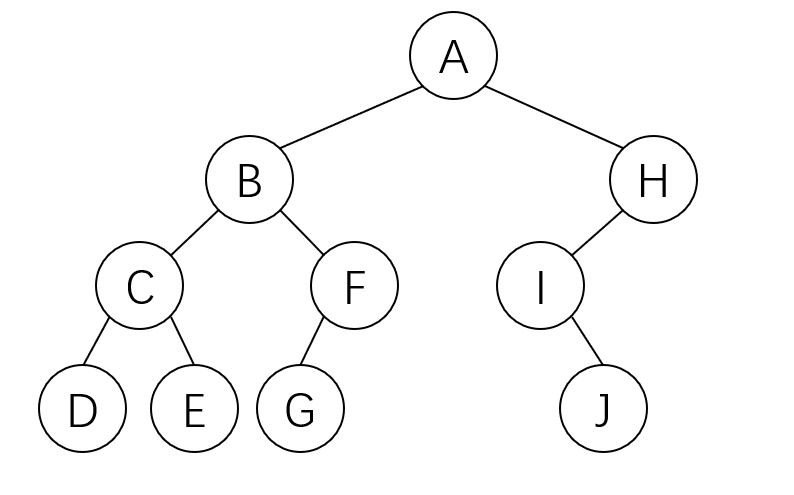
\includegraphics[width=.5\linewidth]{binary_tree.png}
\end{figure}
\begin{enumerate}[(a)]
\item Pre-order depth-first traversal. (4 points)
\begin{solution}
%Write your answer here.
A B C D E F G H I J
\end{solution}

\item Post-order depth-first traversal. (4 points)
\begin{solution}
%Write your answer here.
D E C G F B J I H A
\end{solution}

\item In-order depth-first traversal. (4 points)
\begin{solution}
%Write your answer here.
D C E B G F A I J H
\end{solution}

\item Level-order traversal. (4 points)
\begin{solution}
%Write your answer here.
A B H C F I D E G J
\end{solution}

\end{enumerate}


\subsection{Draw The Tree (10 points)}
\begin{enumerate}[a)]
\item Now we have a specific binary tree, but we only know some of its traversals. Its pre-order traversal is: \textbf{FBADCEGIH}, and its in-order traversal is: \textbf{ABCDEFGHI}. Then please \textbf{draw out the binary tree} and show its \textbf{post-order traversal}. (4 points)

\begin{solution}
%Write your answer here.
\begin{figure}[H]
    \centering
    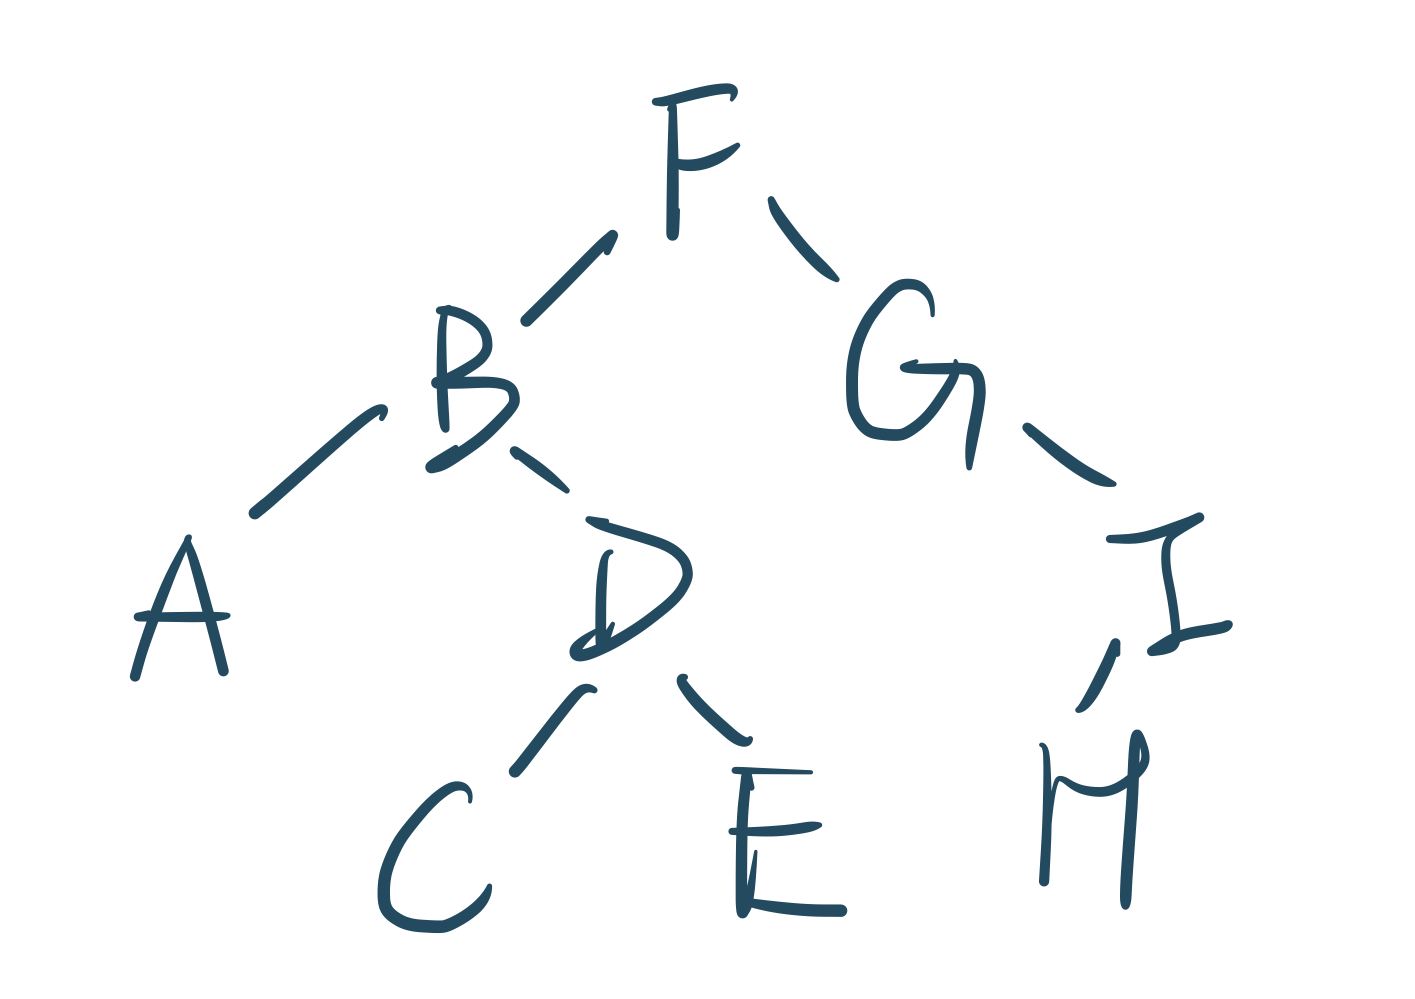
\includegraphics[width=.5\linewidth]{1.png}
\end{figure}
\textbf{post-order traversal}: A C E D B H I G F
\end{solution}
\item Now we have a specific binary tree, but we only know some of its traversals. Its post-order traversal is: \textbf{FEKLJIHG}, and its in-order traversal is: \textbf{EFGHIKJL}. Then please \textbf{draw out the binary tree} and show its \textbf{pre-order traversal}. (4 points)

\begin{solution}
%Write your answer here.
\begin{figure}[H]
    \centering
    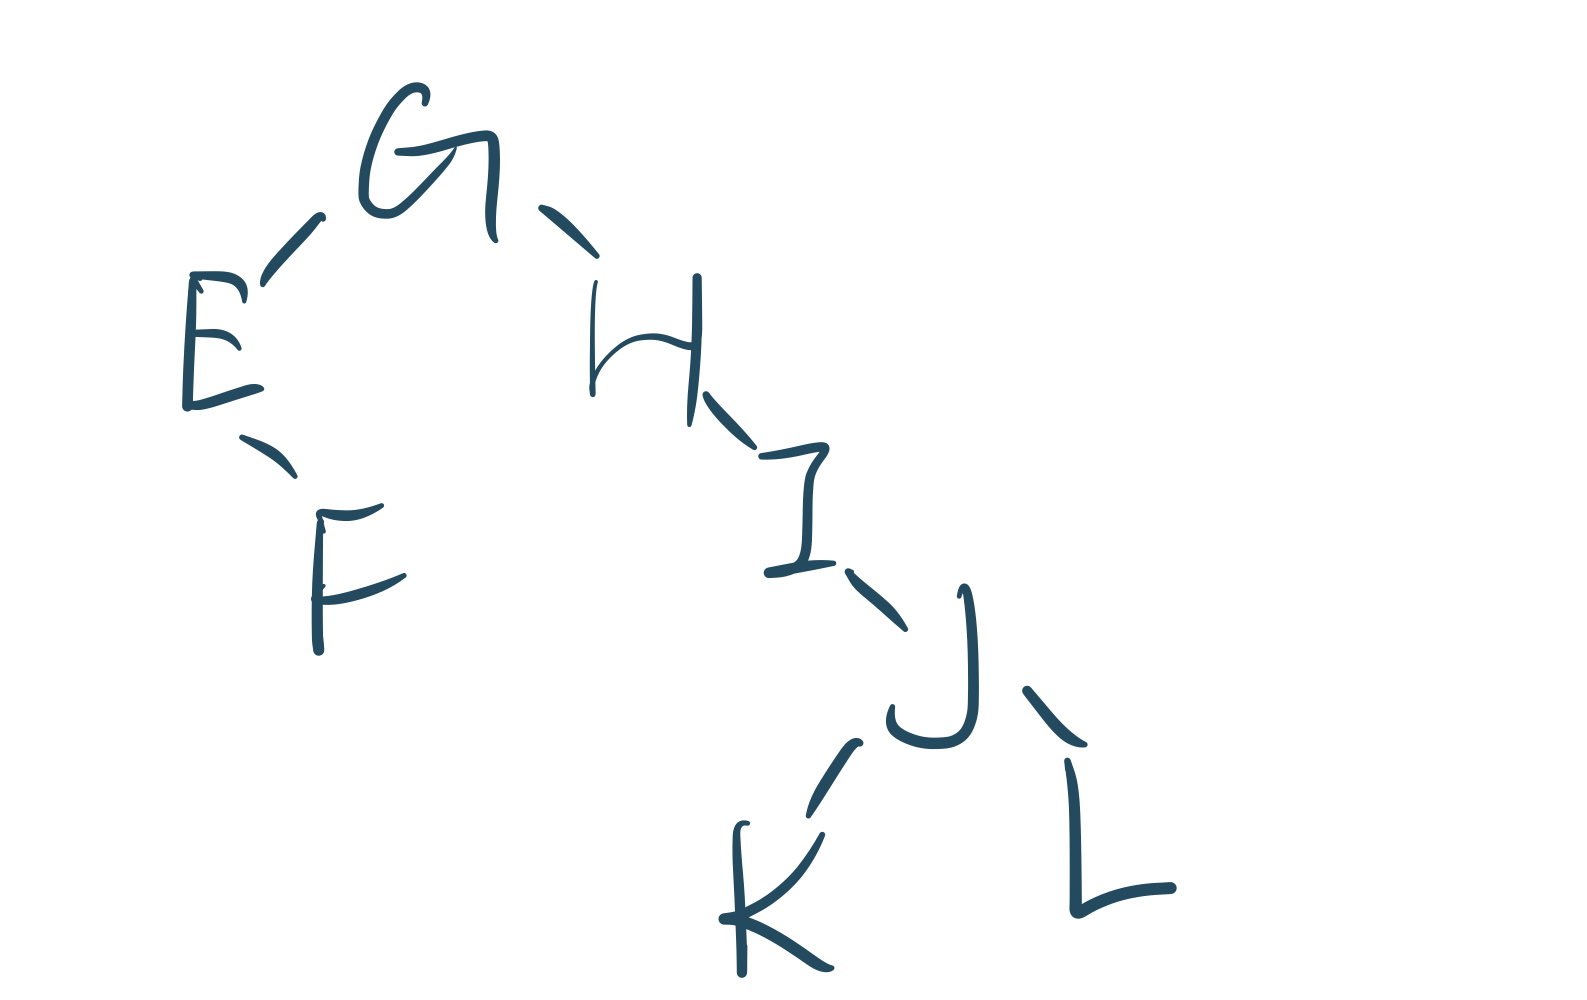
\includegraphics[width=.5\linewidth]{2.png}
\end{figure}
\textbf{pre-order traversal}: G E F H I J K L
\end{solution}

\item Now students are required to draw out the binary tree according to the given traversals: Its pre-order traversal is: \textbf{EACBDGF}, and its post-order traversal is: \textbf{BDCAFGE}. Then please \textbf{draw out the binary tree} and show its \textbf{pre-order traversal}.

Roihn and Conedx both provide their plot of the unknown trees. 
\begin{figure}[H]
\centering
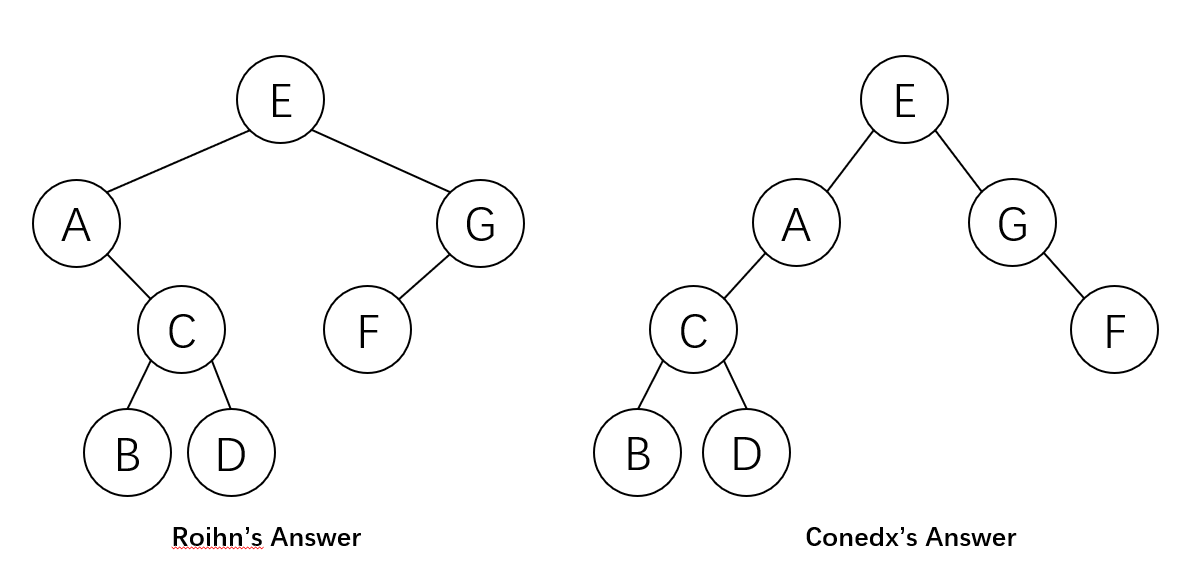
\includegraphics[width=.8\linewidth]{two_ans.png}
\end{figure}

Their answers are totally different, but seem to be both correct. Can you explain why such a case happens? (2 points)

\begin{solution}
%Write your answer here.
\par
When doing pre-order traversal, we visit the node, then left subtree, then right subtree. So when there is only one child and we just write, for example, \textbf{XY}, we cannot make sure that \textbf{X} is the left or right child of \textbf{Y}. Similarly, for \textbf{YX} in post-order, we are stil not sure. In this case, we can only know that \textbf{C} and \textbf{F} are children of \textbf{A} and \textbf{G} respectively, but cannot know whether they are left or right children.
\end{solution}

\end{enumerate}


\section{True or False (20 points)}
Please judge whether the following statements are \textbf{TRUE} or \textbf{FALSE}. You can briefly state your reason if you would like to get partial points. Each question takes 2 points.
	\begin{enumerate}[a)]
		\item A complete tree is a tree where every node has either 0 or 2 children.
		\begin{solution}
%Write your answer here.
False.
\end{solution}
		\item A complete tree is a tree where every level except the last is necessarily filled, and in the last level, nodes are filled in from left to right.
\begin{solution}
%Write your answer here.
True.
\end{solution}
		\item Heapsort has worst-case $\Theta(n \log n)$ time complexity.
		\begin{solution}
%Write your answer here.
True.
\end{solution}
		\item  Percolate-up has an average-case time complexity of $\Theta(\log n)$.
\begin{solution}
%Write your answer here.
True.
\end{solution}
		\item Dequeue is done by simply removing the root.
\begin{solution}
%Write your answer here.
False.
\end{solution}
		\item Enqueue in a min-heap is done by inserting the element at the end, and then calling percolate-up.
\begin{solution}
%Write your answer here.
True.
\end{solution}
		\item $[2, 13, 8, 16,  13, 10, 40, 25, 17]$ is a representation of a min-heap.
\begin{solution}
%Write your answer here.
True.
\end{solution}
		\item $[3, 5, 6, 7, 12, 15, 14, 9, 10, 11]$ is a representation of a min-heap.
\begin{solution}
%Write your answer here.
False.
\end{solution}
		\item  Proceeding from the bottom of the heap to the top, while repeatedly calling percolateDown() can initialize a min-heap.
\begin{solution}
%Write your answer here.
True.
\end{solution}
		\item Proceeding from the top of the heap to the bottom, while repeatedly calling percolateUp() can not initialize a min-heap.
		\begin{solution}
%Write your answer here.
False.
\end{solution}
	\end{enumerate}

\section{Hea---------p! (23 points)}
Consider a min-heap represented by the following array:
\begin{align*}
\{63,74,67,85,91,94,72,88\}
\end{align*}

Perform the following operations using the algorithms for binary heaps discussed in lecture. Ensure that the heap property is restored at the end of every individual operation.

For the following operations, please briefly describe what and how you use the given functions: \textbf{percolateUp()} and \textbf{percolateDown()}, and show the result of the heap after each operation in either tree form or array form.

\begin{enumerate}[a)]
\item Push the value of 60 into this min-heap. (4 points)
\begin{solution}
%Write your answer here.
\par
Add 60 to the end: \\
\{63, 74, 67, 85, 91, 94, 72, 88, 60\}
\par
To maintain the property, call \textbf{percolateUp()}: \\
\{63, 74, 67, 60, 91, 94, 72, 88, 85\} \\
\{63, 60, 67, 74, 91, 94, 72, 88, 85\} \\
\{60, 63, 67, 74, 91, 94, 72, 88, 85\}
\end{solution}

\item Push the value of 79 into this min-heap. (4 points)
\begin{solution}
%Write your answer here.
\par
Add 60 to the end: \\
\{60, 63, 67, 74, 91, 94, 72, 88, 85, 79\}
\par
To maintain the property, call \textbf{percolateUp()}: \\
\{60, 63, 67, 74, 79, 94, 72, 88, 85, 91\}
\end{solution}

\item Update element 85 to have a value of 58 (Suppose you have the access to each element). (5 points)
\begin{solution}
%Write your answer here.
\par
85 -> 58: \\
\{60, 63, 67, 74, 79, 94, 72, 88, 58, 91\}
\par
To maintain the property, call \textbf{percolateUp()}: \\
\{60, 63, 67, 58, 79, 94, 72, 88, 74, 91\} \\
\{60, 58, 67, 63, 79, 94, 72, 88, 74, 91\}  \\
\{58, 60, 67, 63, 79, 94, 72, 88, 74, 91\}
\end{solution}

\item Remove the min element from the heap. (5 points)
\begin{solution}
%Write your answer here.
\par
Copy the root (58) and return. Cut the last leaf and copy it to the root: \\
\{91, 60, 67, 63, 79, 94, 72, 88, 74\}
\par
To maintain the property, call \textbf{percolateDown()}: \\
\{60, 91, 67, 63, 79, 94, 72, 88, 74\} \\
\{60, 63, 67, 91, 79, 94, 72, 88, 74\} \\
\{60, 63, 67, 74, 79, 94, 72, 88, 91\}
\end{solution}

\item Update element 67 to have a value of 96 (Suppose you have the access to each element) (5 points)
\begin{solution}
%Write your answer here.
\par
67 -> 96: \\
\{91, 60, 96, 63, 79, 94, 72, 88, 74\}
\par
To maintain the property, call \textbf{percolateDown()}: \\
\{91, 60, 72, 63, 79, 94, 96, 88, 74\}
\end{solution}

\end{enumerate}

\section{Binary Search Tree (30 points)}
\subsection{Simple simulation (14 points)}

Perform the following operations to construct a binary search tree. Show the result of the BST after each operation in either tree form or array form.

\begin{enumerate}[a)]
\item Insert 24, 29, 22, 25, 19, 32, 15, 37 (3 points)
\begin{solution}
%Write your answer here.
\begin{figure}[H]
    \centering
    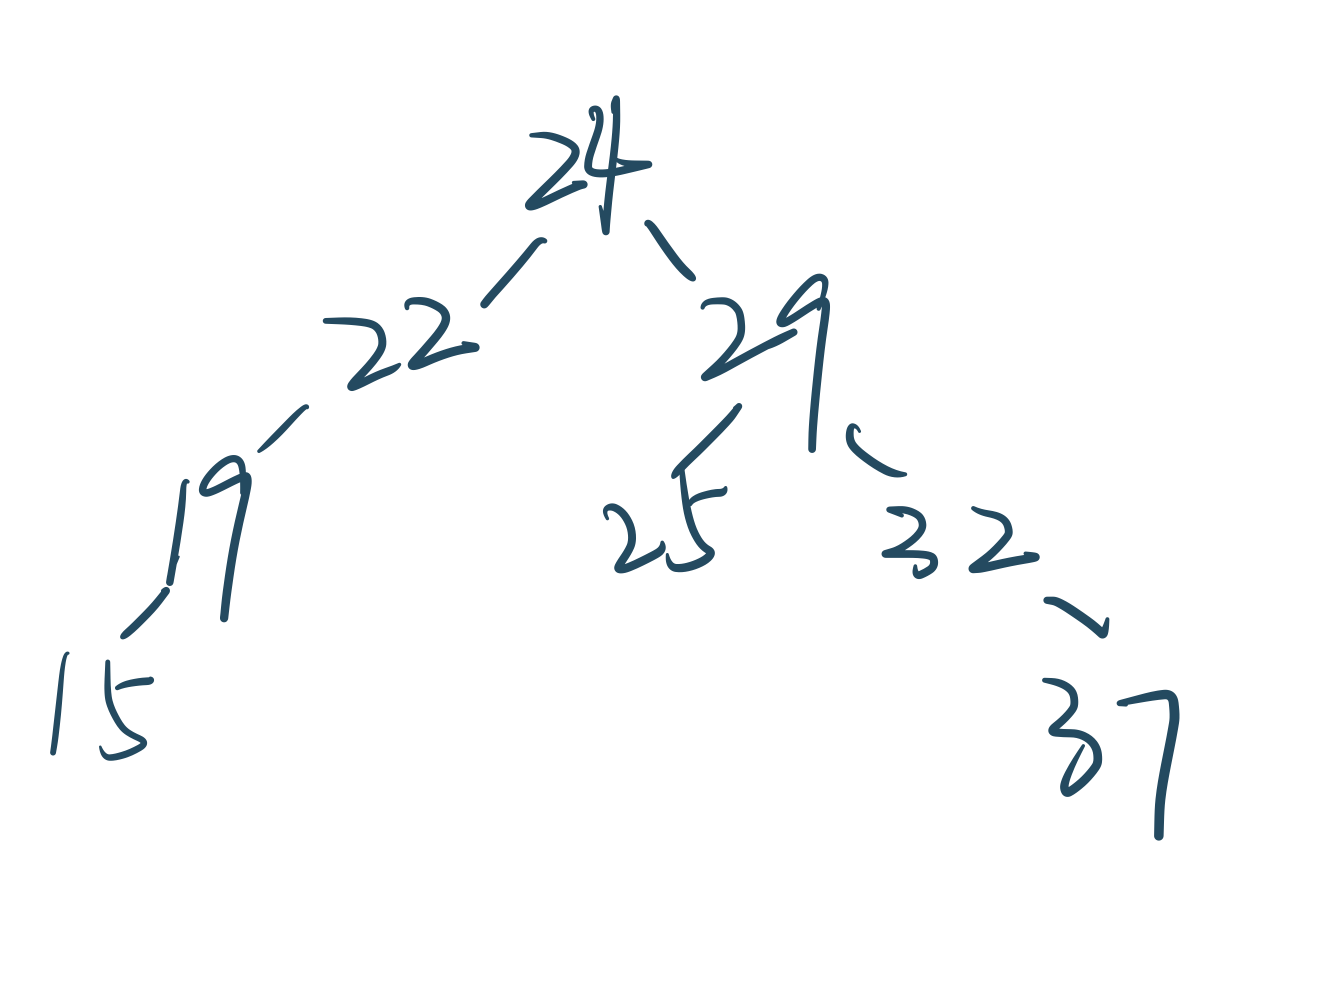
\includegraphics[width=.5\linewidth]{3.png}
\end{figure}
\end{solution}

\item Delete 22 (3 points)
\begin{solution}
%Write your answer here.
\begin{figure}[H]
    \centering
    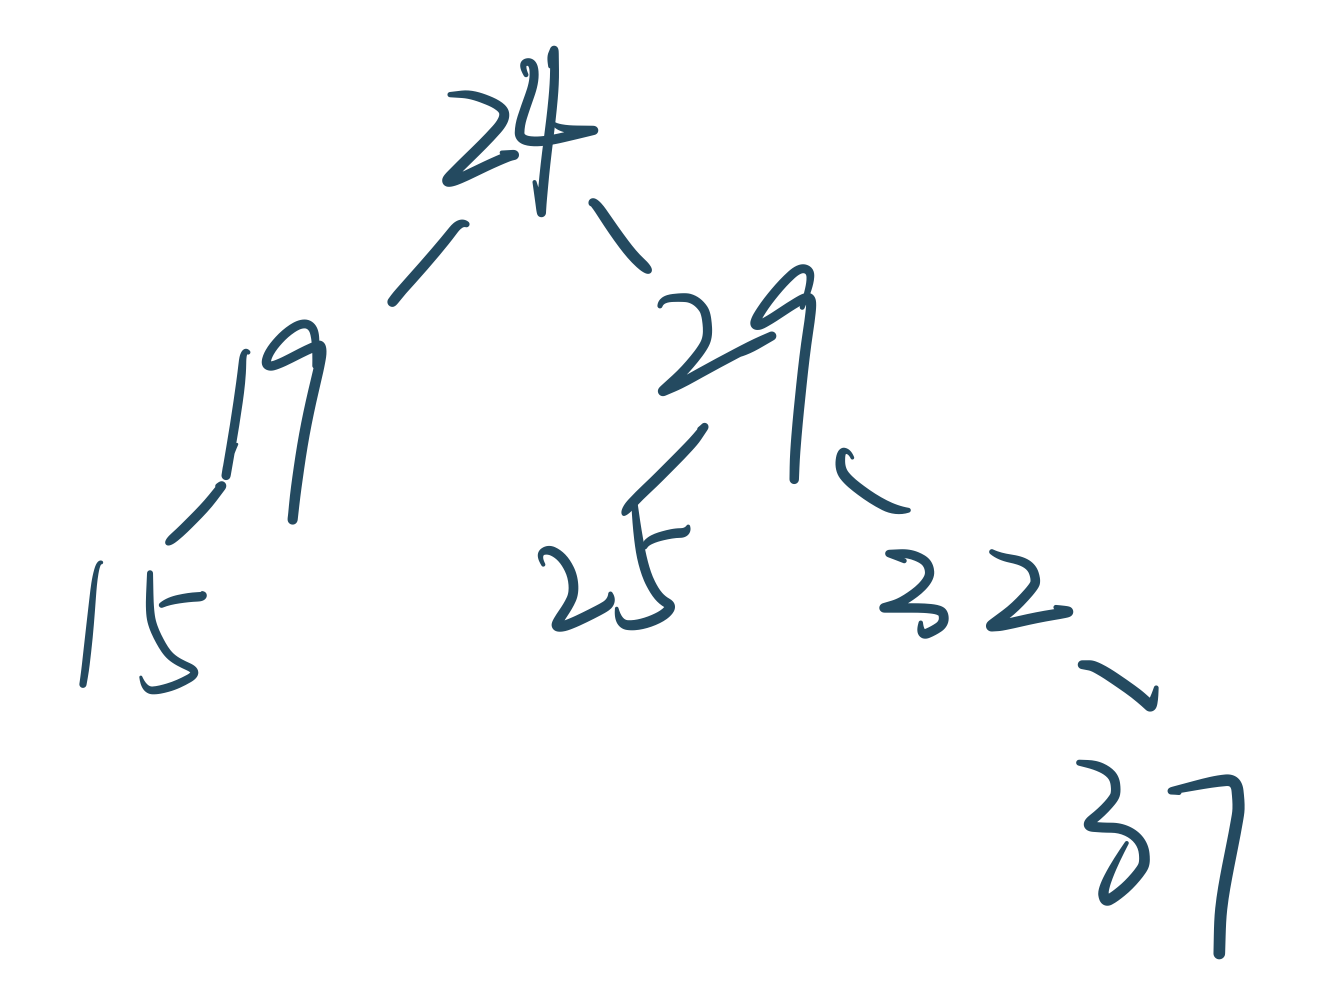
\includegraphics[width=.4\linewidth]{4.png}
\end{figure}
\end{solution}

\item Delete 29 (3 points)
\begin{solution}
%Write your answer here.
\begin{figure}[H]
    \centering
    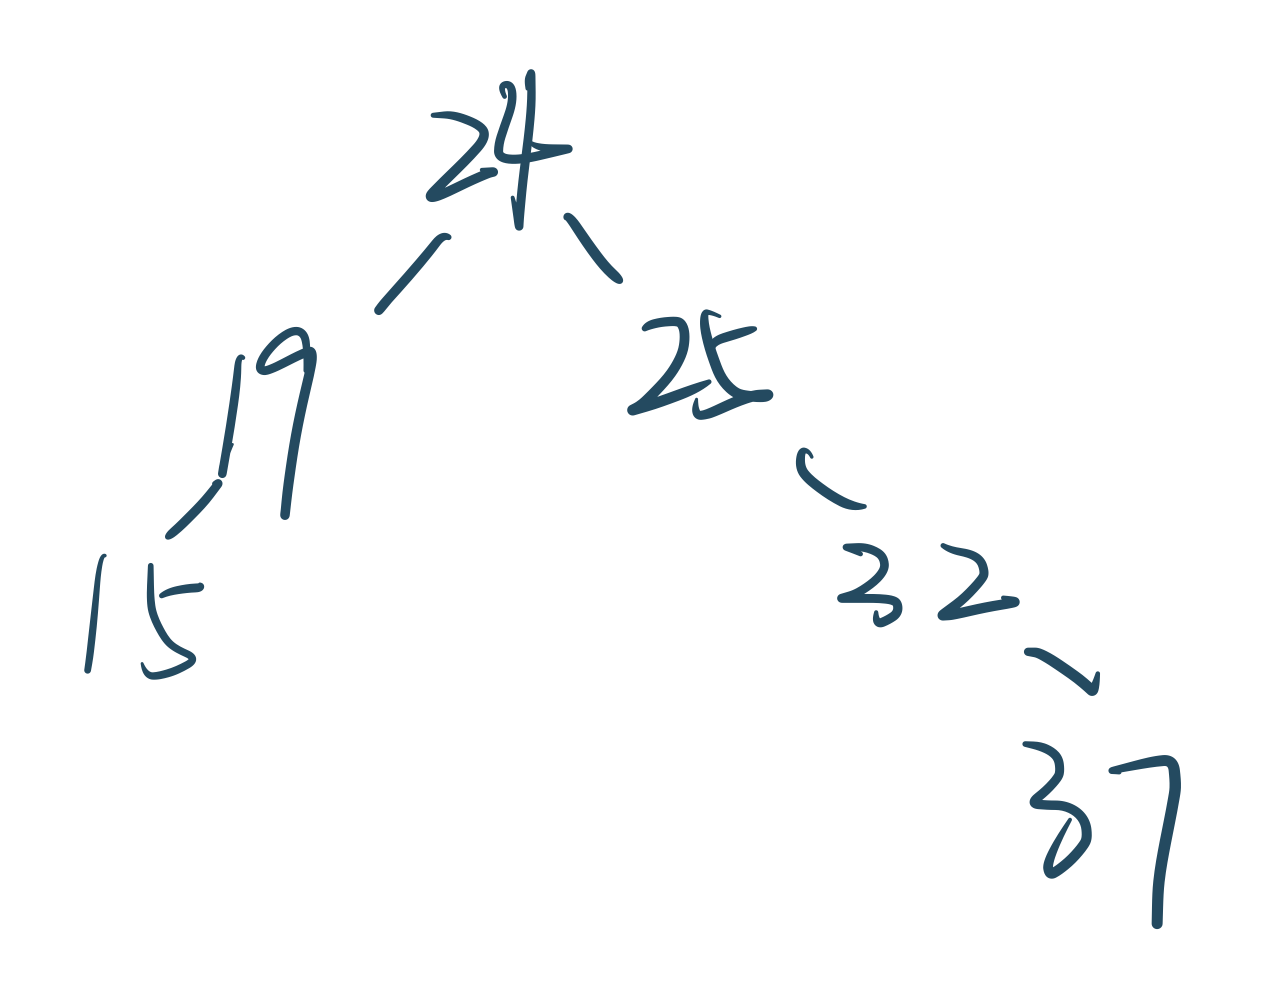
\includegraphics[width=.4\linewidth]{5.png}
\end{figure}
\end{solution}

\item Insert 22 (3 points)
\begin{solution}
%Write your answer here.
\begin{figure}[H]
    \centering
    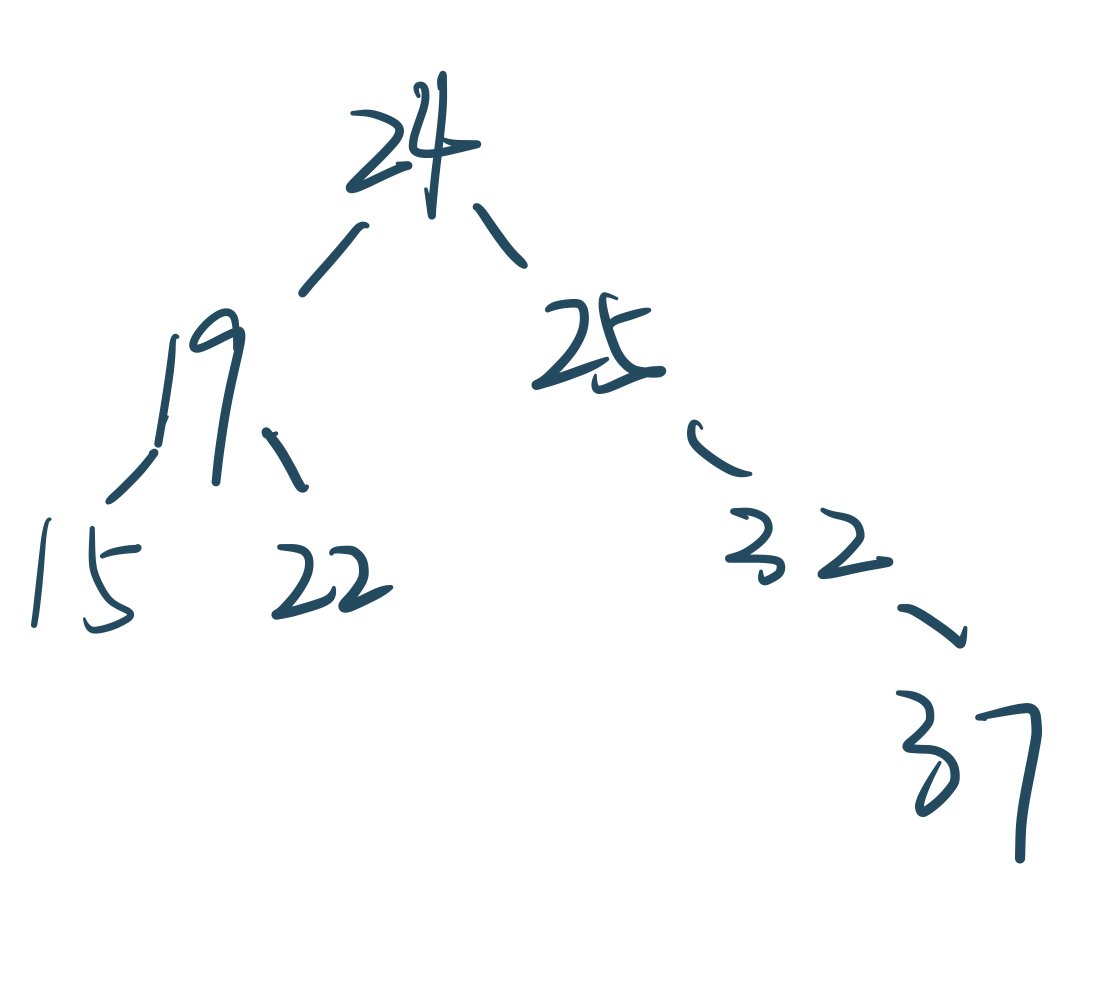
\includegraphics[width=.4\linewidth]{6.png}
\end{figure}
\end{solution}

\item What is the inorder predessor of node 25? What is the inorder sucessor of node 32? (2 points)
\begin{solution}
%Write your answer here.
\par
inorder predessor of node 25: 24\\
inorder sucessor of node 32: 37
\end{solution}


\end{enumerate}

\subsection{Let's BST! (16 points)}
\begin{enumerate}[a)]
\item Suppose that in a binary search tree, when a node with two children is deleted, it is replaced by its inorder successor. Given a pointer to the node to be deleted, what is the time complexity of finding the inorder successor in the average case, if the tree contains $n$ nodes? Briefly explain your answer. (4 points)
\begin{solution}
%Write your answer here.
\par
$O(\log n)$ \\
Assume that the node we are going to delete is a subtree containing $m$ elements (including itself). Then it takes average $O(\log m)$ to find its inorder successor. \\
To calculate the average time complexity regarding $n$, consider the average number $M$ of elements that a subtree of a $n$-element tree can contain. \\
Consider a perfect BST, with $n$ elements and height $h$. We can find that:
 $$M=\frac{2^{h}}{2^{h}-1}(h+\frac{1}{2^{h}}-1)=O(h)=O(\log n)$$
Then, the average time complexity in this case is: $O(\log M)=O(\log n)$. \\
Among all the possible cases, the more unbalanced, the less likely that it will occur. So roughly speaking, the average case should be balanced, nearly a perfect BST. So the average time complexity among all cases should be $O(\log n)$.
\end{solution}

\item
Suppose that you want to insert 12 distinct elements into a binary search tree. How many worst-case trees are possible for these 12 elements? (6 points)
\begin{solution}
%Write your answer here.
\par
In the worst case, the tree becomes a linked list (each node has only one child or none). So the root should be the smallest or the largest element, or it will have two children. And then, each following node should be the largest or smallest element among the remained elements, or there will be two children. For example, for \{1, 2, 5\}, if we insert 4, indicating that 5 is not the smallest or largest element in the remained elements, then 2 will have two children. \\
Then we have:
$$N = 2^{11}$$
possible worst-case trees. Each node has two choices, except for the last one.
\end{solution}

\item
Consider a tree that satisfies the following conditions:
\begin{enumerate}[1.]
\item The tree is a binary search tree of integers.
\item The number of elements in the root node's left and right subtrees are the same.
\item There are no duplicate values in the tree.
\item The first element of an inorder traversal of the tree is 11.
\item The last element of an inorder traversal of the tree is 24.
\item The last element of a postorder traversal of the tree is 16.
\end{enumerate}

What is the largest possible integer you can attain by summing up all the values in a tree that satisfies the above constraints? (6 points)

\begin{solution}
%Write your answer here.
\par
According to 4, 5, 6, we can know that the smallest element is $11$, the largest is $24$, and the root is $16$. \\
Since it's a BST, and no duplicate values, all the elements in the root's left subtree should be smaller than $16$, and all the elements in the root's right subtree should be bigger than $16$. \\
According to 1, we just consider integers. There are 5 integers in $[11,16)$ and 8 integers in $(16,24]$. According to 2, and to make the sum be the largest, we take the largest 5 elements in both side. \\
The sum is:
$$11+12+13+14+15+16+20+21+22+23+24 = 191$$
\end{solution}


\end{enumerate}

\section*{Reference}
Assignment 3, VE281, FA2020, UMJI-SJTU.



\end{document}











